\section{Experiment Subjects}
\label{sec:experimentSubjects}

\subsection{Explanation Methods}
\label{subsec:explanationMethods}
We use the following saliency methods for our experiments: Occlusion as the single perturbation-based method, seven gradient-based methods including Vanilla Gradient or Saliency, GradientSHAP, Guided Backpropagation, Guided GradCAM, Integrated Gradients, DeepLift, and LRP. Specific hyperparameters were required for some of these methods, which we specified as follows:
\begin{itemize}
    \item For Occlusion: we use an $8\times8$ occlusion window and a $4\times4$ stride.
    \item For Integrated Gradients and GradientSHAP: we use a baseline generated from a uniform distribution on the interval $[0, 1)$.
\end{itemize}

\subsection{Black boxes}
We opted to use XAI methods on the InceptionV3 \cite{inceptionv3} and Resnet101 \cite{resnet101} architectures for several reasons. One primary reason is that these models are based on Convolutional Neural Networks (CNNs), which are necessary for certain model-specific XAI techniques like Class Activation Mapping (CAM) and Grad-CAM. These techniques leverage the inherent structure and characteristics of CNNs to produce visual explanations and highlight significant regions in an image. Additionally, we chose InceptionV3 and Resnet101 because of their demonstrated performance in previous work conducted by Narin, Ali et al. in their study on COVID-19 detection using X-ray images \cite{covidXray}. Although these models do not have sustainable G-ops (giga operations per second), they have shown good performance in specific applications, particularly in the medical domain. By applying XAI methods to these architectures, we aim to gain a deeper understanding of their performance in medical imaging tasks.

\subsubsection{Residual Network - 101}
\label{subsubsec:resnet101}
ResNet-101 is a convolutional neural network architecture that was introduced by He et al. in 2015 \cite{resnet101}. The residual network was developed to address the challenge of training very deep neural networks by utilizing residual connections.

The key idea of residual networks lies in their residual block design, which allows for the effective training of extremely deep models. In traditional deep networks, the increasing depth often leads to performance degradation due to the difficulty of learning mappings from input to output. A residual network solves this issue by introducing skip connections, or shortcut connections, that allow the network to learn residual mappings. By propagating gradients through these shortcuts, the model can effectively capture residual information and learn more efficiently.

\begin{figure}
\centering
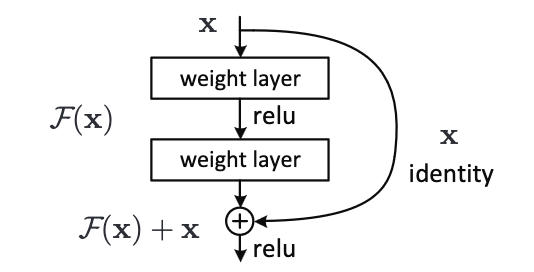
\includegraphics[width=13cm]{images/blackboxes/res_block.png}
\caption{Residual Block Diagram. Source \cite{resnet101}}
\end{figure}

The ResNet-101 architecture consists of 101 layers, including convolutional layers, pooling layers, and fully connected layers. The model employs a bottleneck structure in each residual block, reducing computational complexity while maintaining performance. The architecture has demonstrated impressive performance on various image recognition tasks, including the ImageNet Large-Scale Visual Recognition Challenge (ILSVRC) \cite{imageNet}, where it achieved state-of-the-art results.  With its ability to effectively train very deep models, ResNet-101 has contributed significantly to advancements in the field of deep learning and medical image analysis.

\begin{figure}
\centering
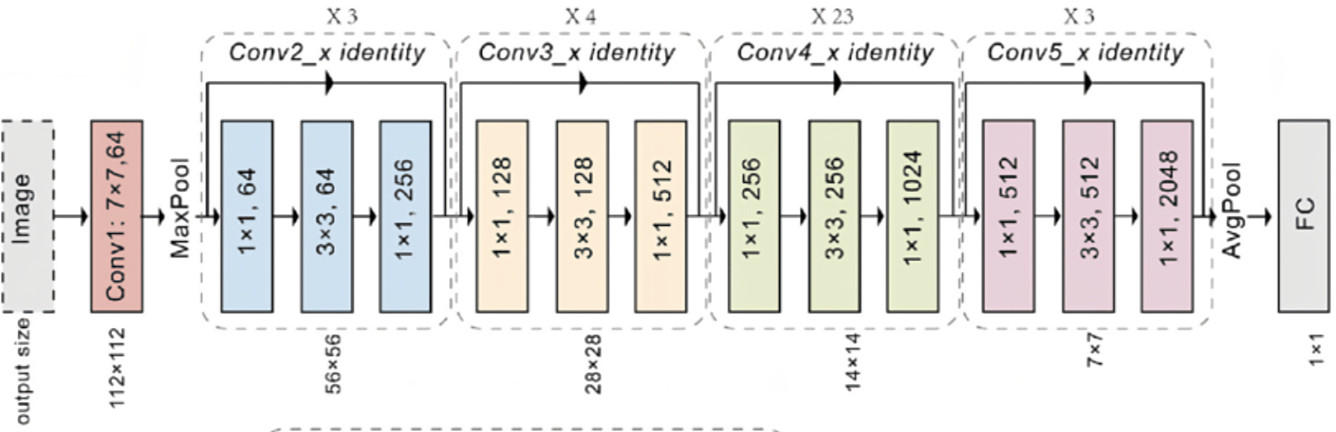
\includegraphics[width=13cm]{images/blackboxes/resnet101.png}
\caption{Resnet101 Architecture Diagram. Source \cite{resnet101Diagram}}
\end{figure}


\subsubsection{InceptionV3}
The InceptionV1 model addresses the problem of overfitting that arises when using deep layers of convolutions by employing parallel layers of multiple filter sizes at the same level. This wider architecture prevents the model from becoming excessively deep, mitigating overfitting risks.

\begin{figure}
\centering
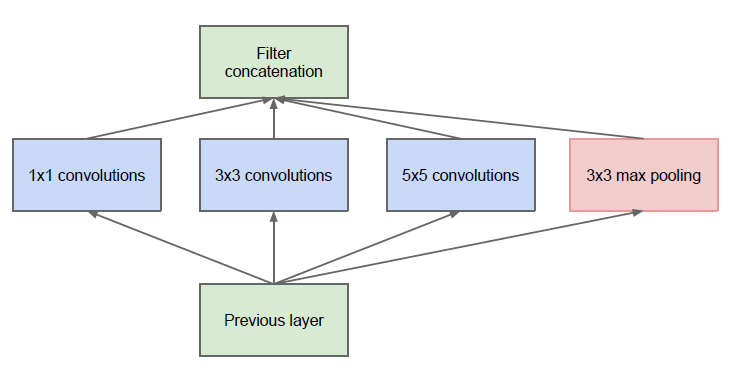
\includegraphics[width=13cm]{images/blackboxes/inception_module.png}
\caption{Naive Form of Inception Block. Source \cite{resnet101}}
\end{figure}

InceptionV3 further enhances the original Inception design with several modifications. One key modification is the factorization of the 5×5 convolutional layer into two 3$\times$3 convolutional layers, reducing computational costs while maintaining expressive power. Another improvement involves spatial factorization, replacing n×n convolutions with a 1×n convolution followed by an n×1 convolution. This two-layer solution reduces computational expenses by 33\% when the number of input and output filters is equal.

\begin{figure}
\centering
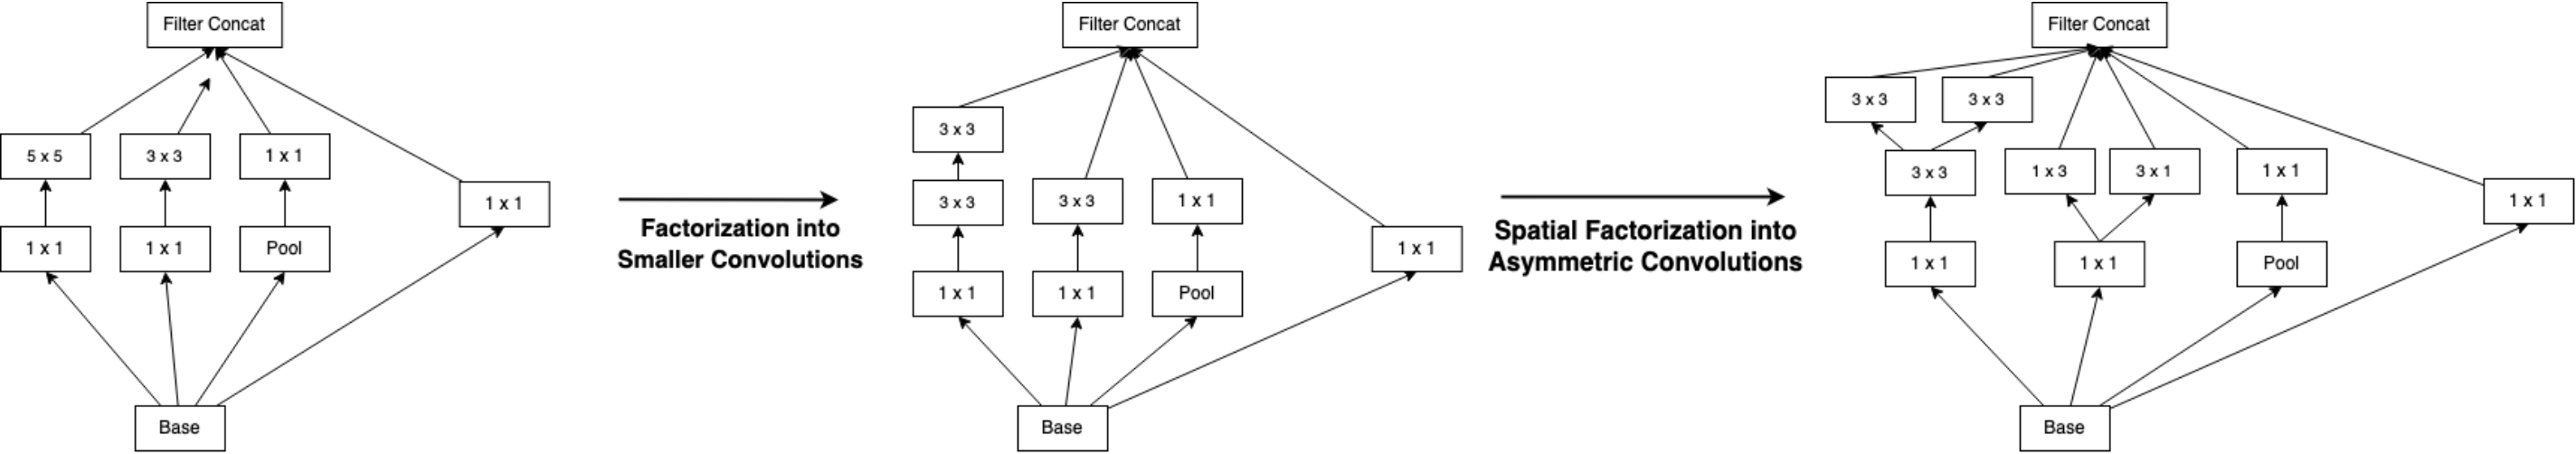
\includegraphics[width=13cm]{images/blackboxes/inception3_ideas.png}
\caption{Some major optimizations of InceptionV3 model. Source \cite{inceptionv3}}
\end{figure}

The InceptionV3 model also introduces the use of auxiliary classifiers, which act as regularization techniques for the architecture. These auxiliary classifiers aid in training by providing additional supervision during the learning process. Additionally, efficient grid size reduction is achieved through the utilization of two parallel blocks of convolution and pooling, which are later concatenated.

\begin{figure}
\centering
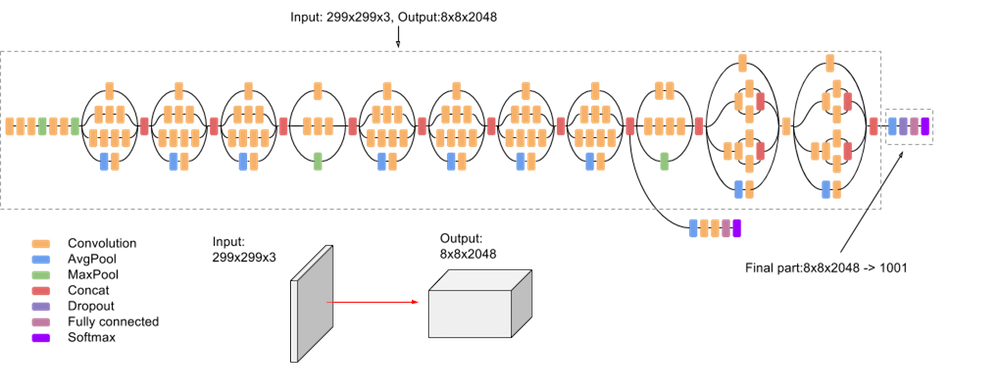
\includegraphics[width=13cm]{images/blackboxes/inceptionv3.png}
\caption{InceptionV3 Architecture. Source \cite{inceptionv3}}
\end{figure}

Another modification is the reduction in the grid size of feature maps by employing two parallel blocks of convolution and pooling. This design allows for a more efficient reduction in grid size while maintaining the expressive power of the network. Specifically, if we start with a $w\times w$ grid with $k$ filters, after reduction, it results in a $w/2\times w/2$ grid with $2k$ filters. By expanding the activation dimension in this manner, InceptionV3 ensures more efficient use of network capacity and computation. The two parallel blocks of convolution and pooling operate independently, capturing different types of information from the input. These blocks are then concatenated, combining the extracted features in a complementary way

These modifications in InceptionV3 enable improved performance and computational efficiency, making it a powerful model for various computer vision tasks. The Inception family of models has contributed significantly to the field of deep learning, demonstrating the effectiveness of wider architectures and factorization techniques in achieving state-of-the-art results.